\documentclass{beamer}
\usetheme{Boadilla}

\usepackage[absolute,overlay]{textpos}
\usepackage{graphicx}
\usepackage{tikz}
\usepackage{comment}

\title{Digital Forensics}
\subtitle{File System Forensics Masterclass}
\author{Fraser Brown}
\institute{Heriot-Watt University}
\date{March 28, 2018}

\graphicspath{{../figures/}}


%%%%%%%%%%%%%%%%%%%%%%%%%%%%%%%%%%%%%%%%%%%%%%%%%%%%%%%%%%%%%%%%%%%%%%
% LaTeX Overlay Generator - Annotated Figures v0.0.1
% Created with http://ff.cx/latex-overlay-generator/
% If this generator saves you time, consider donating 5,- EUR! :-)
%%%%%%%%%%%%%%%%%%%%%%%%%%%%%%%%%%%%%%%%%%%%%%%%%%%%%%%%%%%%%%%%%%%%%%
%\annotatedFigureBoxCustom{bottom-left}{top-right}{label}{label-position}{box-color}{label-color}{border-color}{text-color}
\newcommand*\annotatedFigureBoxCustom[8]{\draw[#5,thin,rounded corners] (#1) rectangle (#2);\node at (#4) [fill=#6,thick,shape=circle,draw=#7,inner sep=0.5,font=\sffamily,text=#8] {\tiny #3};}
%\annotatedFigureBox{bottom-left}{top-right}{label}{label-position}
\newcommand*\annotatedFigureBox[4]{\annotatedFigureBoxCustom{#1}{#2}{#3}{#4}{white}{white}{black}{black}}
\newcommand*\annotatedFigureText[4]{\node[draw=none, anchor=south west, text=#2, inner sep=0, text width=#3\linewidth, font=\sffamily] at (#1){\tiny #4};}
\newenvironment {annotatedFigure}[1]{\centering\begin{tikzpicture}
\node[anchor=south west,inner sep=0] (image) at (0,0) { #1};\begin{scope}[x={(image.south east)},y={(image.north west)}]}{\end{scope}\end{tikzpicture}}
%%%%%%%%%%%%%%%%%%%%%%%%%%%%%%%%%%%%%%%%%%%%%%%%%%%%%%%%%%%%%%%%%%%%%%



\begin{document}

\begin{frame}
\titlepage
\end{frame}

\begin{frame}
\frametitle{What is this Masterclass?}
This masterclass aims to give an overview of digital forensics and provide practical experience through a lecture and lab combination.\\
\vspace{\baselineskip}
The materials will be structured as follows:
\begin{enumerate}
	\item Lecture (EM1.01) 10:15-11:15
	\item Lab (EM2.50) 11:15 - 13:15
\end{enumerate}
\vspace{\baselineskip}
\textbf{Lecture and Lab Resources:} \\

\url{http://www2.macs.hw.ac.uk/~fmb30/digital-forensics/}
\end{frame}

\begin{frame}[allowframebreaks]
\frametitle{Lab Overview}
\textbf{The Scenario:}\\
You are digital forensics investigators working on a data information leakage case for a client.\\
\vspace{\baselineskip}

Your hypothetical team has given you a USB stick recovered from the person suspected of leaking information. You will analyse the file system and try to prove if they have leaked information.\\


\begin{itemize}
	\item Set up a Lab Environment using Kali Linux
	\item Create/Gather a Forensic image of the USB in question.
	\item Perform automated data carving
	\item Gather file system information.
	\item Keyword searching of unallocated space {\&} extraction of related (deleted) files.
	\item Recover and confirm evidence using metadata pointers.
\end{itemize}

\textbf{Reserouce Credits:}\\
The USB resources we will be using in today's lab are from the \textit{National Institute of Standards and Technology (NIST)} as part of their \textit{Computer Forensic Reference Data Sets (CFReDS)}\footnote{\url{https://www.cfreds.nist.gov/}}.\\
\vspace{\baselineskip}

The rest of the resources and a can be found here:\\
\url{https://www.cfreds.nist.gov/data_leakage_case/data-leakage-case.html}
\end{frame}

\begin{frame}
\section*{Lecture Overview}
\frametitle{Lecture Overview}
\tableofcontents
\end{frame}

\begin{frame}
	\frametitle{What is Digital Forensics?}
	\section{What is Digital Forensics?}
%	\begin{itemize}
%		\item Digital forensics is a pulls from both cyber security and forensic science fields.
%	\end{itemize}
	\begin{block}{Digital Forensics:}
		``Computer [Digital] Forensics is the practice of \textit{determining the past actions that have taken place on a computer system} using forensic techniques and understanding artefacts.'' - David Cowen
	\end{block}
		
	\begin{block}{Artefact:}
		``An Artefact is a \textit{reproducible} file, setting or system change that occurs every time an application or operating system performs a specific action'' - David Cowen
	\end{block}

	The artefacts we will be dealing with in the lab are files and file systems.
\end{frame}

\begin{frame}[allowframebreaks]
	\frametitle{Why File System Analysis?}
	\subsection*{Why File System Analysis?}
	\begin{itemize}
		\item There are many different forms of digital forensic analysis:
			\begin{itemize}
				\item Network Analysis,
				\item Live memory (RAM) Analysis, 
				\item File system analysis, 
				\item Database Analysis,
				\item Application/OS Analysis
			\end{itemize}
			\item File system analysis allows:
			\begin{itemize}
				\item Introduction to a new field (digital forensics).
				\item A different perspective on computer science knowledge we already have.
				\item Insight into how files relate to memory, and what creation and deletion features actual do.
			\end{itemize}
	\end{itemize}
	\begin{figure}
		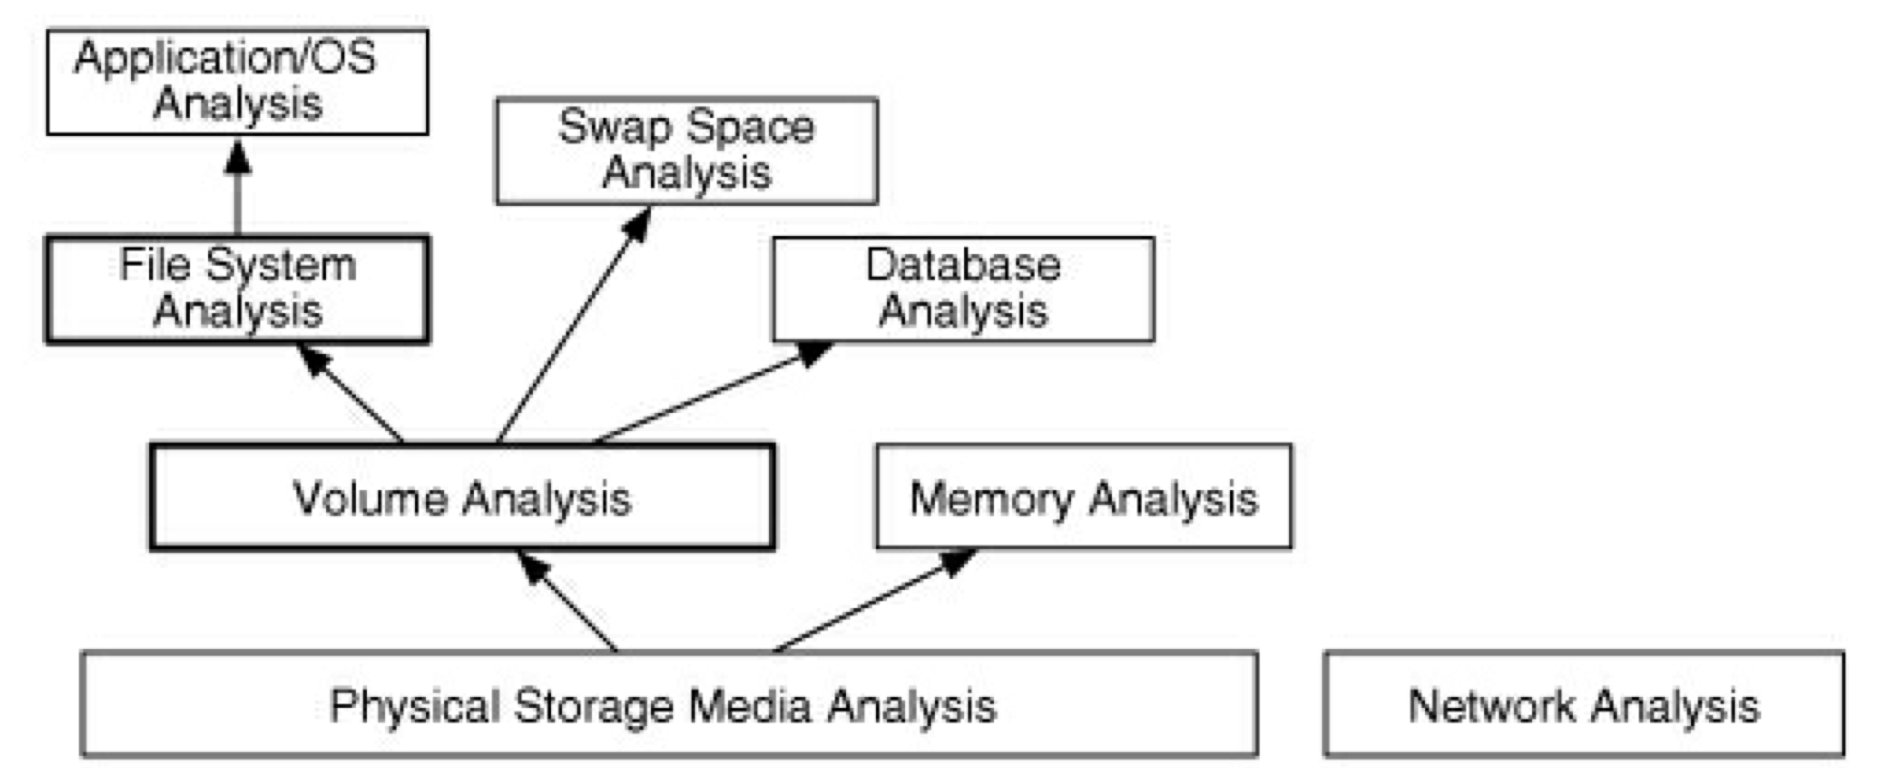
\includegraphics[scale=0.3]{digital-data-analysis-layers-BrianCarrier}
		\caption{Layers of Analysis\footnote{Carrier, Brian. File System Forensic Analysis (Kindle Location 619). Pearson Education. Kindle Edition.}} 

	\end{figure}
\end{frame}

\begin{frame}% Title Page
	\section{Forensic Process}
	\begin{center}
		\Huge\textbf{Forensic Process}
	\end{center}
\end{frame}

\begin{frame}
	\frametitle{Forensic Process}
	\textit{Digital forensics results can be used in a court of law} therefore \textbf{accuracy}, \textbf{integrity} and an \textbf{unbiased approach} towards evidence is required.\\
	Traditional approaches towards evidence handling and procedure are shared between traditional and digital forensics.   
	\begin{block}{Scientific Method}
		Defining a hypothesis based on evidence then proceeding search for evidence which disproves our hypothesis.
	\end{block}
	\begin{block}{Digital Forensic Investigation}
	``A digital forensic investigation is a process that \textit{uses science
     and technology} to \textit{analyse digital objects} and that \textbf{develops and
     tests theories,} which can be entered into a court of law, to
     \textit{answer questions about events that occurred}.'' - Brian Carrier\footnote{\tiny{Carrier, Brian. File System Forensic Analysis (Kindle Locations 480-481). Pearson Education. Kindle Edition.}} 
	\end{block}
\end{frame}

\begin{frame}
	\frametitle{Digital Crime Scene Investigation Process Overview}
	\subsection*{Digital Crime Scene Investigation Process Overview}
	There are three major areas in digital crime scene investigations:
	\begin{itemize}
		\item System Preservation
			\begin{itemize}
				\item Write Blockers,
				\item Cryptographic Hashes,
				\item Proper Evidence Handling,
				\item Photographic Evidence of a crime scene/workstation.
			\end{itemize}
		\item Evidence Searching
			\begin{itemize}
				\item Data Carving,
				\item Metadata information gathering.
				\item Deleted file recovery. 
			\end{itemize}
		\item Event Reconstruction
			\begin{itemize}
				\item Time line creation
				\item Gathering/providing reliably recreatable evidence. 
			\end{itemize}
	\end{itemize}
\end{frame}

\begin{frame}
	\frametitle{PICL Guidelines}
	\subsection*{PICL Guidelines}
	While each forensic investigator/team may have their own procedures and work flow the PICL guidelines below provide a good starting structure:\\
	\vspace{\baselineskip}
	\begin{itemize}
		\item \textbf{Preservation}:\\	 Preservation of the system being investigated.
		\item \textbf{Isolation}:\\	 Keeping analysis environment is separate from both the suspect data and the outside world.
		\item \textbf{Correlation}:\\	 Correlate data with other independent sources. Reduces risk of forged data.
		\item \textbf{Logging}:\\	 Log/document your actions. This helps identify what searches you have not yet conducted and what your results were.
	\end{itemize}
\end{frame}

%\begin{frame}
%	\frametitle{Analysis Types}
%	\subsection*{Analysis Types}
%	\begin{block}{Live Analysis:}
%		``A live analysis occurs when you use the operating system or other resources of the system being investigated to find evidence.'' - Brian Carrier\footnote{\tiny{Carrier, Brian. File System Forensic Analysis (Kindle Locations 495-496). Pearson Education. Kindle Edition.}}
%	\end{block}
%
%	\begin{block}{Dead Analysis:}
%		``A dead analysis occurs when you are running trusted applications in a trusted operating system to find evidence.'' - Brian Carrier\footnote{\tiny{Carrier, Brian. File System Forensic Analysis (Kindle Locations 496-497). Pearson Education. Kindle Edition. }}
%	\end{block}
%\end{frame}

\begin{frame} %Title Page
	\section{Forensic Imaging}
	\begin{center}
		\Huge\textbf{Forensic Imaging}
	\end{center}
\end{frame}

\begin{frame}
	\frametitle{Evidence Acquisition/Imaging}
	\begin{itemize}
		\item In order to perform analysis on digital artefacts a forensic \textbf{duplicate} of the media must be created.
		\item \textit{Forensic Duplicates} are \textbf{bit-for-bit copies of the original disk} and can encompass the full disk or a single partition. 
		\item This process is known as \textbf{imaging} or \textbf{acquisition}.
		\item Contents of a disk are always changing therefore \textbf{Write Blockers} are used to preserve the disk state.
		\item \textbf{Cryptographic hash functions} such as \texttt{SHA-256, SHA-1, MD5} are used to \textbf{verify} the image against the original artefact.
	\end{itemize}
\end{frame}

\begin{frame}
	\frametitle{Image Types}
	\subsection*{Image Types}
	\begin{itemize}
		\item Raw Format (\texttt{.dd} \texttt{.raw} \texttt{.img})
		\begin{itemize}
			\item Only contain data from the original artifact
			\item Metadata on image is not included however can be generated into a separate file by tools. (guymager, TSK)
			\item Tools: \texttt{dd}, \texttt{dcfldd}, \texttt{dd\_rescue}, \texttt{rdd}, \texttt{df3dd}, \texttt{guymager}
		\end{itemize}
		\item EnCase Evidence Format (Expert Witness \texttt{.E01})
		\begin{itemize}
			\item Expert Witness images use headers and footers to hold metadata about the image.
			\item Metatdata can include: drive type, source disk OS, timestamps, hashes, CRCs over blocks.
		\end{itemize}
	\end{itemize}
\end{frame}

\begin{frame}
	\frametitle{Write Blockers}
	\subsection*{Write Blockers}
	\begin{block}{Write Blockers}
			Are hardware or software devices that allow gathering of information without damaging the disk contents by blocking write commands but allowing read commands.
	\end{block}
	\begin{itemize}
		\item Write Blockers are customisable:
			\begin{itemize}
				\item Blocking of all or specific commands.
				\item Can control the read and write speed.
			\end{itemize}
		\item Write Blockers come in two forms:
			\begin{itemize}
				\item \emph{Native}: Same interface for input and output e.g. IDE-to-IDE
				\item \emph{Tailgate}: uses different interfaces for input and output e.g. firewire/USB-to-SATA
			\end{itemize}
		\end{itemize}
\end{frame}

\begin{frame}
	\frametitle{Imaging Challenges with Solid State Drives (SSD)}
	\subsection*{Imaging Challenges}
	While an SSD can be imaged with the same tools as a traditional hard disk drive (HDD), there are technology specific issues that cause problems for forensic investigators.
	\begin{itemize}
		\item \textbf{Program-Erase cycles}
			\begin{itemize}
				\item Sequence of events that result in data being written to a solid state flash memory cell, then erased and rewritten (e.g flash memory USB sticks). 
				\item These P/E cycles result in a \textit{small amount of physical damage to the medium}, which can result in \textbf{bad sectors}.
			\end{itemize}
		\item \textbf{Wear Levelling}
			\begin{itemize}
				\item Prolongs the life of solid state/flash memory.
				\item Distributes rewrites evenly across the medium, so no single block dies prematurely.
			\end{itemize}
		\item These two technologies due to the evolution of memory results in unallocated space being overwritten earlier than it would on a HDD. This could overwrite valuable hidden information by accident
	\end{itemize}
\end{frame}

\begin{frame}% Title Page
	\section{File Systems}
	\begin{center}
		\Huge\textbf{File Systems}
	\end{center}
\end{frame}

\begin{frame}[allowframebreaks]
	\frametitle{What are File Systems?}
	\begin{block}{File System:}
		File systems manage how data is \textbf{stored} and \textbf{retrieved} in a computer system. They consist of \textbf{structural} and \textbf{user data} which can be organised and understood by users and computers.
	\end{block}
	
	\begin{itemize}
		\item File system architectures (FAT32, Ext3 etc.) provide \textit{different methods of tracking data on physical media}, each has their own data structures and look up tables. % and allocation methods.
		\\
		
		\item Modern operating systems \textit{contain support for many different file systems} providing an interface with physical storage, defining things like allocation methods. 
	\end{itemize}
	
	\newpage
	File systems are made up of 2/3 layers:
	\begin{enumerate}
		\item\textbf{Logical Layer}: Provides a user application level API for commands such as read, write and chmod etc.
		\item\textbf{Virtual Layer} (\textit{optional}): Allows access to multiple physical file systems e.g. block based: FAT32, NTFS or network based: NFS
		\item\textbf{Physical Layer}: Interacts with hardware, performing block and memory management and interacting with device drivers etc.
	\end{enumerate}
\end{frame}

\begin{frame}
	\begin{figure}[h]
		\begin{minipage}[c]{0.6\textwidth}
			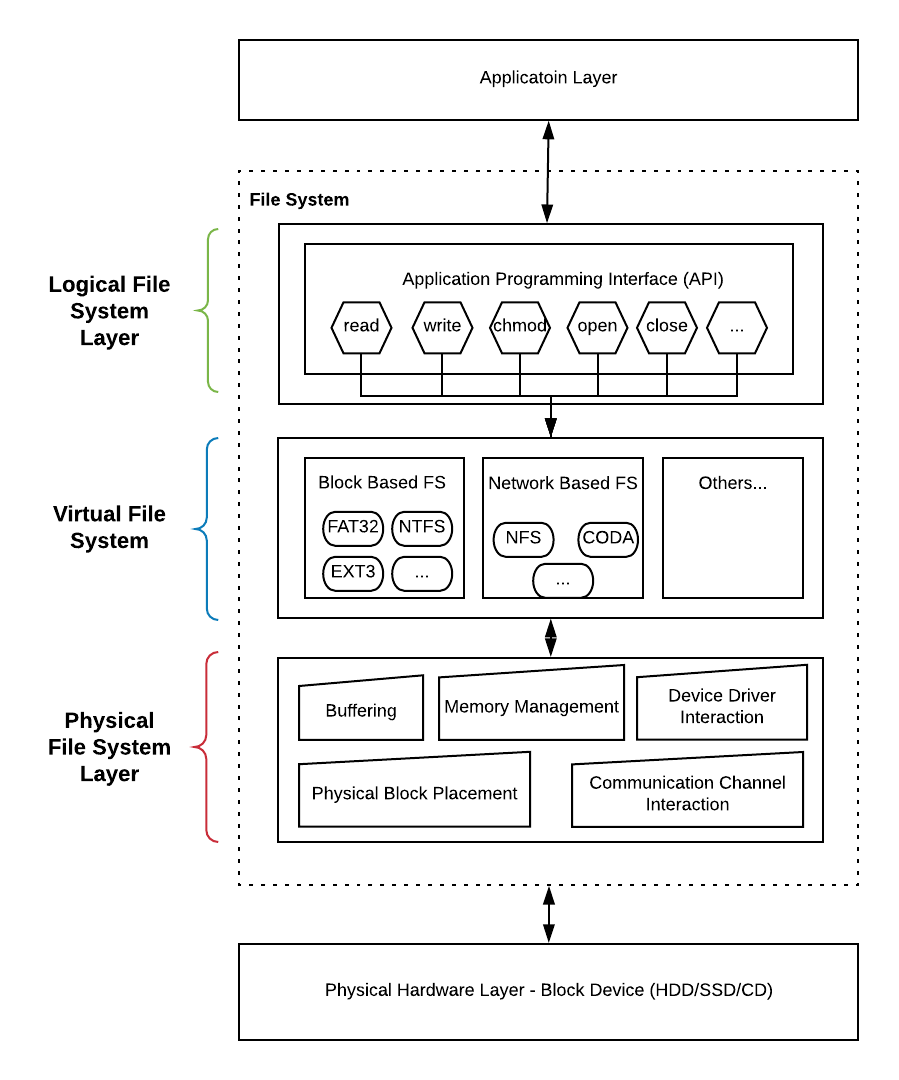
\includegraphics[scale=0.53]{abstract-fs-diagram}
		\end{minipage}\hfill
		\begin{minipage}[c]{0.37\textwidth}
			\caption{Abstract Diagram of a File System on a Computer}
			\label{fig:abstract-fs-diagram}	
		\end{minipage}
	\end{figure}
\end{frame}

\begin{frame}
	\frametitle{File Systems Terminology}
	\subsection*{File System Terminology}
	\begin{itemize}
		\item{\textbf{Sector}}:\\ Smallest addressable section of memory, which holds static amount of data (512/2048/4096-bytes)
		%\item\textbf{Volume}:\\ 
		\item\textbf{INode}:\\ Data structure in a file system that contains meta data (a.k.a Meta Data Pointers/Structures)
		\item\textbf{Data Unit}:\\ Standard sized container for storing \textit{content} data,which consists of multiple \textbf{sectors}. Different file systems have different names for these data units e.g. (Cluster or Block). 
	\end{itemize}
\end{frame}

\begin{frame}
	\frametitle{File System Data Categories}
	\subsection*{File System Data Categories}
	All data in a file system belongs to a data category listed below. This abstract view will be useful for analysing different elements of a file system for evidence and for visualising structures that make up a file on disk.
	\begin{itemize}
		\item \textbf{File System}: \\ Contains file system structure overview and where to find other structures and important data.
		\item \textbf{Content}: \\ Contains data relating to actual file contents, these are usual organised into containers called data units (block/cluster).
		\item \textbf{Meta data}: \\ Data that describes files such as access times, file size, users.
		\item \textbf{File Name}: \\ Contains the data that assigns a name to a file, is used by users instead of a meta data address.
		\item \textbf{Application}: \\ Special features/additional functionality such as quota data or journalling.	
	\end{itemize}	    
\end{frame}

\begin{frame}
	\frametitle{File System Categories Interaction}
	\begin{figure}[h]
		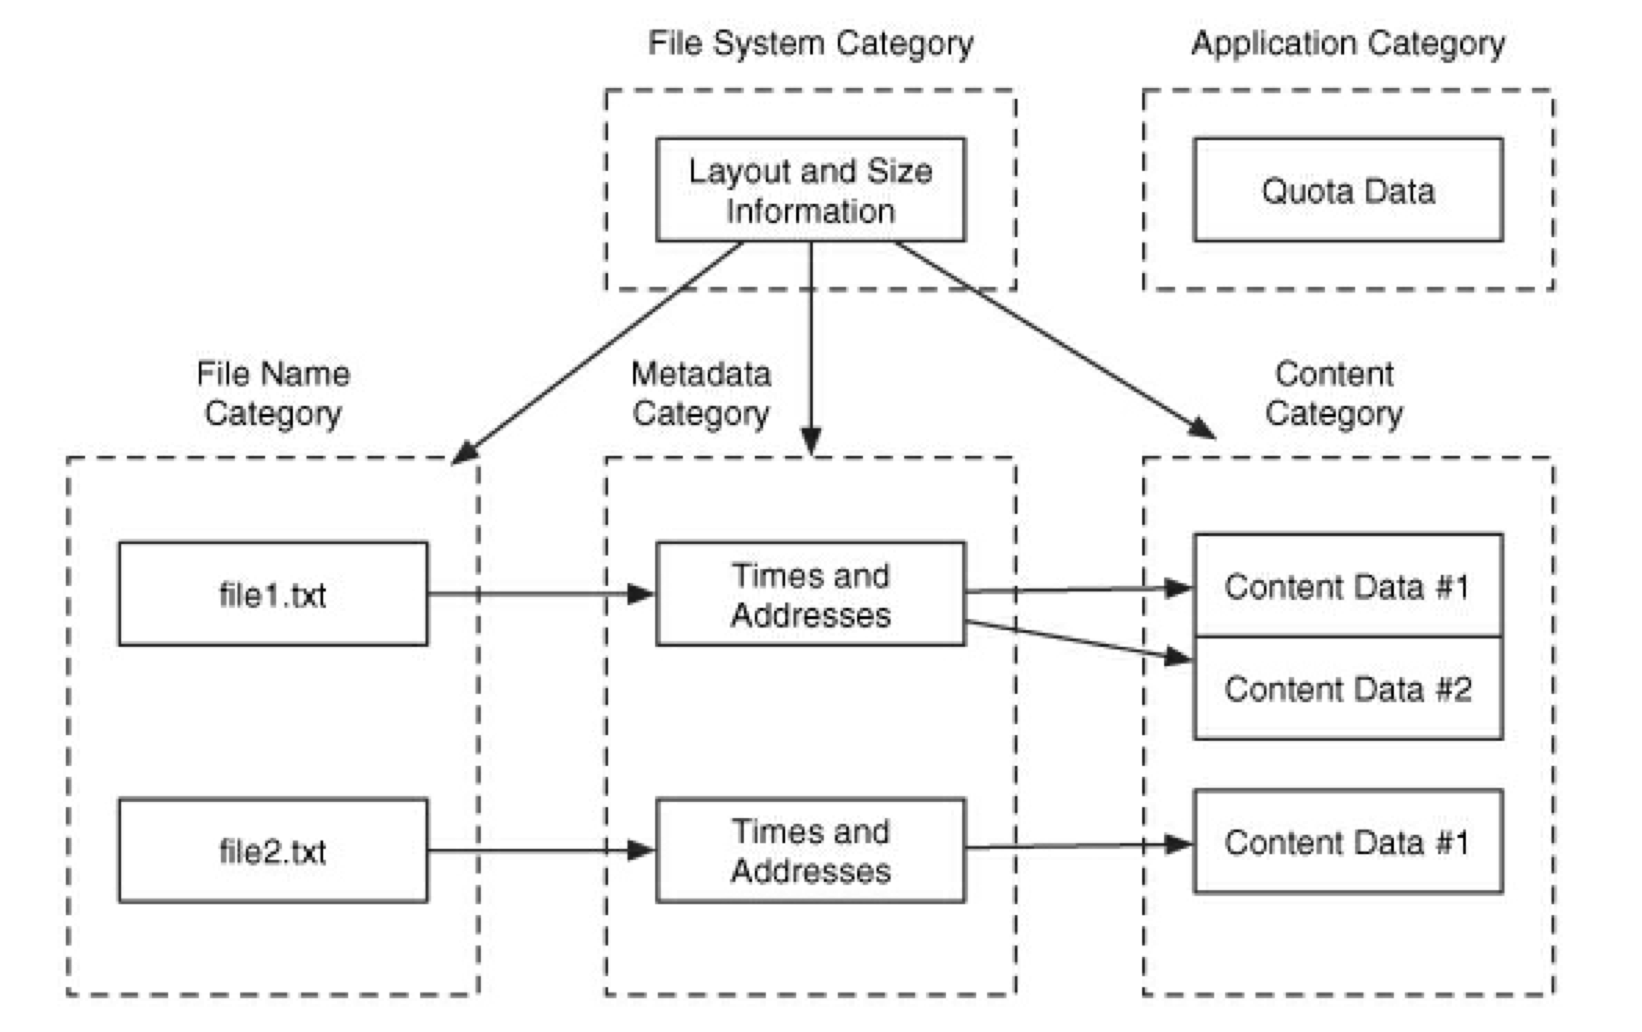
\includegraphics[scale=0.36]{fs-category-interaction-briancarrier}
		\caption{File System Categories Interaction\footnote{\tiny Carrier, Brian. File System Forensic Analysis (Kindle Location 3563). Pearson Education. Kindle Edition. }}
		\label{fig:fs-category-interaction}
	\end{figure}
\end{frame}

\begin{frame}
	\frametitle{File System Categories By Example}
	\begin{figure}[h]
		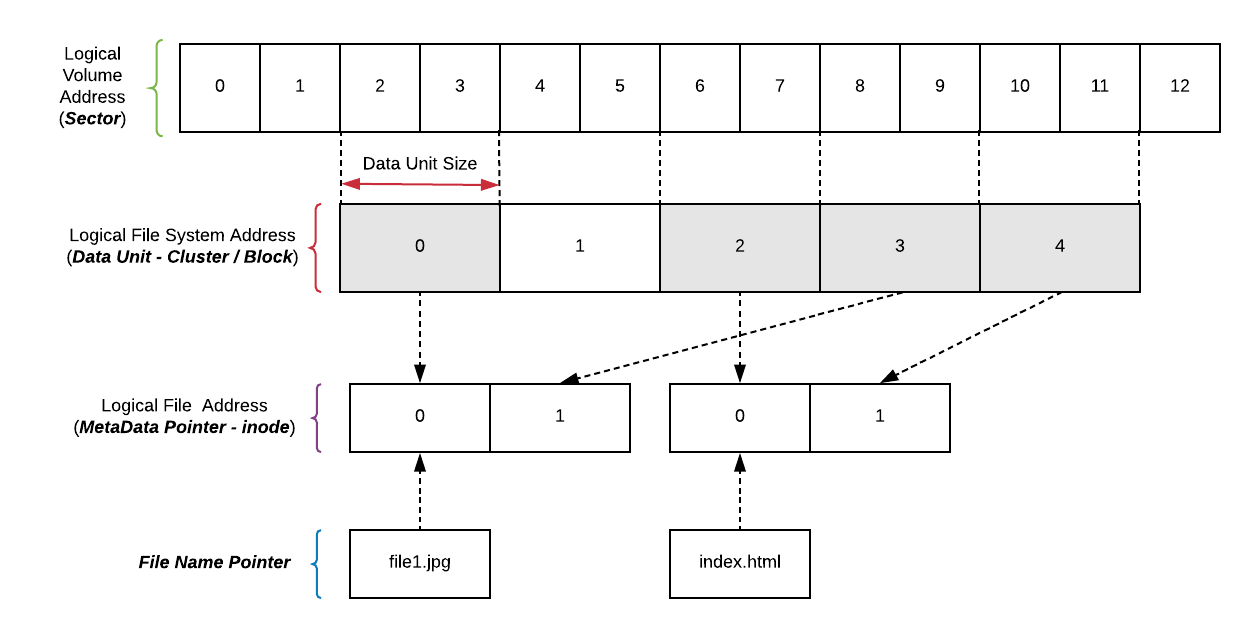
\includegraphics[scale=0.61]{file-system-example}
		\caption{File System Example\footnote{\tiny Carrier, Brian. File System Forensic Analysis (Kindle Location 3797). Pearson Education. Kindle Edition. }}
		\label{fig:fs-example}
	\end{figure}
\end{frame}

\begin{frame}
	\frametitle{File System Architectures}
	\section*{File System Architectures}
	There are numerous file system architectures available, some are operating system specific others are designed to be more universal. \\
	\vspace{\baselineskip}
	Examples include:
	\begin{itemize}
		\item \textbf{FAT} - File Allocation Table (FAT8/16/32) - \textit{Commonly found on Removable Media} 
		\item \textbf{NTFS} - New Technology File System - \textit{Default For Windows}
		\item \textbf{Ext} - Extended File System (Ext2/3/4) - \textit{Default for Linux}
	\end{itemize}
		\vspace{\baselineskip}
	We will focus on FAT32 in this lecture due to the lab being structured around applying forensic techniques on FAT32 formatted removable media.
\end{frame}

\begin{frame}
	\frametitle{File Allocation Table (FAT) Hisotry}
	\section*{File Allocation Table - FAT32}
	\begin{itemize}
		\item File Allocation Table (FAT) file system is a simplistic file system developed for Windows DOS and Windows 9* operating systems. 
		\vspace{\baselineskip}
		\item FAT is supported by both windows and Unix OS's. 
		\vspace{\baselineskip}
		\item FAT was replaced by NTFS as the primary file system of windows in XP era, FAT is now mainly used in SD Cards and USB flash drives.
		\vspace{\baselineskip}
		\item FAT has been extended from the original 8 bit to 32 bit and had derivatives made from it such as exFAT and FAT+
	\end{itemize}	
\end{frame}

\begin{frame}[allowframebreaks]
	\frametitle{FAT32 - Information}
	\subsection*{FAT32}
	\begin{itemize}
		\item Data Units are called \textbf{\textit{Clusters}}
		\item Increased cluster size over FAT8/FAT16 architectures, due to being stored as 32bit values.
		\item FAT32 has two overarching data structures:
			\begin{itemize}
				\item \textbf{File Allocation Table}: \\
				Stores next cluster for a given file, holds allocation status of clusters.
				\item \textbf{Directory Entries}:\\
				One per file/directory which contains: file name , size, starting address of content and other metadata.
			\end{itemize}
		\item The \textit{first cluster address} starts at 2. 
		\item \textbf{\textit{Calculate Sector Address}} of Cluster C:\\ 
			$(C-2)\times (NumberSectorsPerCluster) + (SectorOfCluster2)$
		\item \textbf{Calculate Cluster address} from sector address S:\\
			$((S – SectorOfCluster2) / (NumberSectorsPerClusterr)) + 2$
	\end{itemize}
	\newpage
	Physical Layout of a FAT FS:
	\begin{figure}
		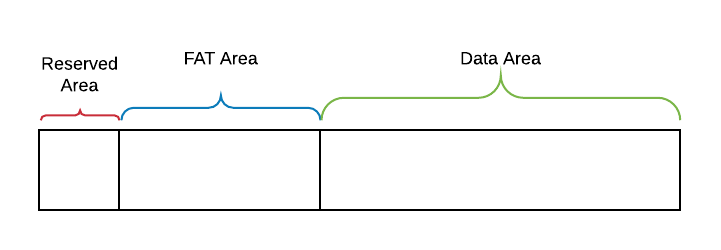
\includegraphics[scale=0.8]{fat-phys-layout}
		\caption{FAT Physical Layout}
		\label{fig:fat-phys-layout}
	\end{figure}
\end{frame}
\begin{frame}% Title Page
	\section{Forensic Tools}
	\begin{center}
		\Huge\textbf{Forensic Tools}\\
		\large\textit{(Used in Accompanying Lab)}
	\end{center}
\end{frame}

\begin{frame}
	\frametitle{Guymager - Forensic Imaging}
	\subsection*{Guymager}
	\begin{block}{Guymager}
		Guymager is a GUI based forensic imaging tool, that allows for the creation of various image types such as Raw (dd) and EnCase (E01).
	\end{block}
	\begin{figure}[h]
		\centering
		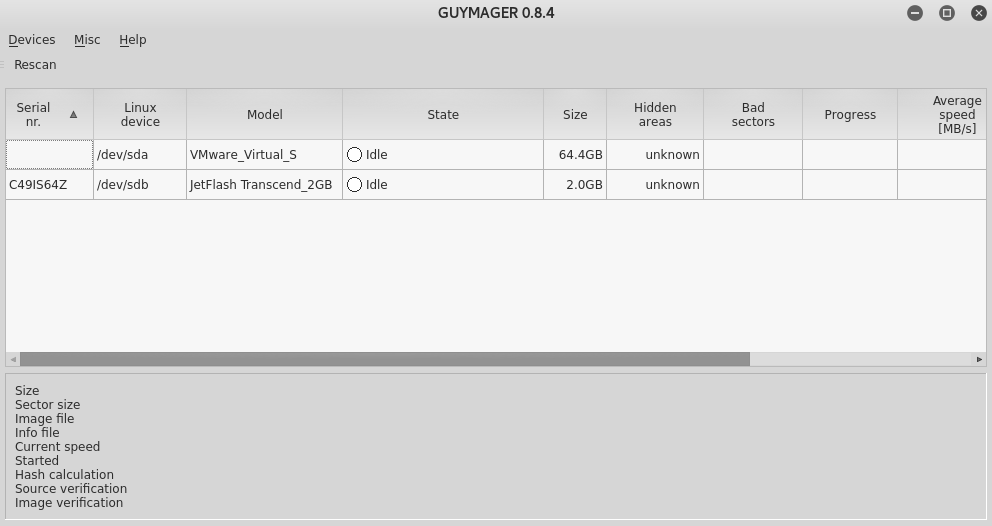
\includegraphics[scale=0.29]{guymager-window}
		\caption{\textit{guymager gui window example}}
		\label{fig:guymager-main-window}
	\end{figure}
\end{frame}

\begin{frame}
	\subsection*{Foremost}
	\frametitle{Foremost - Data Carving}
	\begin{block}{Foremost}
		Foremost is a command line tool that utilises data carving techniques to recover files.
	\end{block}
	\begin{itemize}
		\item \textbf{Data Carving} is a process where files are recovered from a disk image based on common information such as file headers, footers and data structures. 
		\item Performing data carving for large forensic images can be rather tedious if done by hand, tools such as \textbf{Foremost} have been developed to help digital forensic investigators automating this process.
	\end{itemize}
\end{frame}

\begin{frame}
	\subsection*{The Sleuth Kit (TSK)}
	\frametitle{The Sleuth Kit (TSK)\footnote{http://www.sleuthkit.org/}}
	\begin{block}{The Sleuth Kit (TSK)}
	The Sleuth Kit is a series of command line tools that allow users to inspect and analyse disk images and the file systems therein.
	\end{block}
	\begin{itemize}
		\item The tools provided in TSK are divided into the 5 file system categories discussed previously, file system, content (data unit), meta data, file name.
		\item Due to the wide variety of tools within TSK I will discuss those of which we will use in the accompanying lab.
		\item Other features of TSK can befound in the tool overview: \url{http://wiki.sleuthkit.org/index.php?title=TSK_Tool_Overview}
	\end{itemize}
\end{frame}

\begin{frame}% Title Page
	\section{File System Analysis Example}
	\begin{center}
		\Huge\textbf{File System Analysis}\\
		\large\textit{(By Practical Example)}
	\end{center}
\end{frame}

\begin{frame}
	\frametitle{Note About File System Analysis Techniques}
	\section*{File System Analysis Techniques}
	There are many different analysis techniques for each of the aforementioned file system data categories. In the respect of time and scope of the lecture I will only cover the ones that are relevant to the lab materials.
	
	\vspace{\baselineskip}
	
	You may also notice that sometimes the same analysis technique (logical file system searching and viewing) are doable from different categories in a file system. This added redundancy means effective analysis can be performed even if certain data structures don't exists or were removed.
\end{frame}

\begin{frame}
	\frametitle{Initial Volume / Disk Image Enumeration - \texttt{mmls}}
	Before we can get into recovering files or gathering evidence we have to understand the problem space we are working in. TSK provides volume system level tools to aid with this. \texttt{mmls} allows us to display the layout of a disk image/volume.
	\begin{figure}[h!t]
		\begin{annotatedFigure}
			{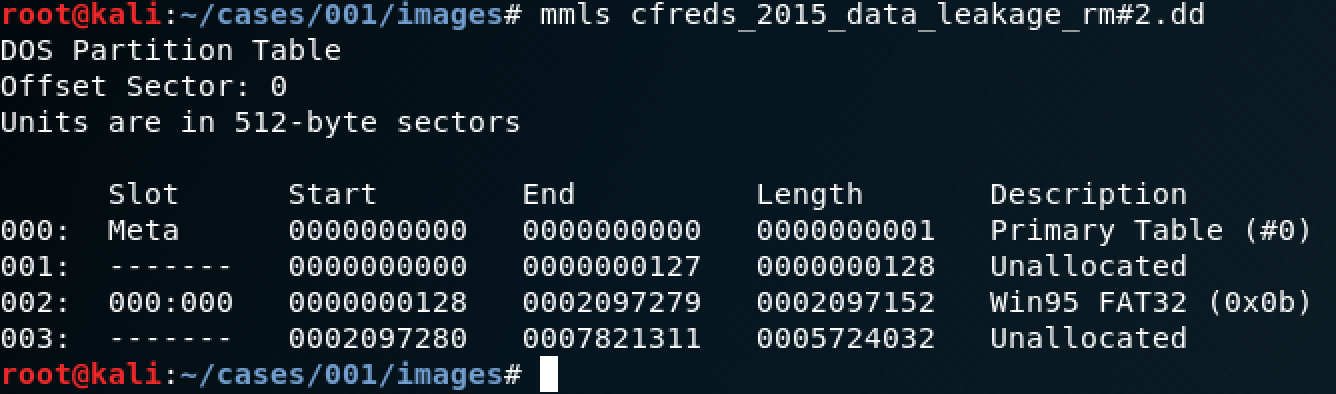
\includegraphics[width=1.0\linewidth]{mmls-output.png}}
			\annotatedFigureBox{0.167,0.6007}{0.3985,0.7417}{B}{0.167,0.6007}%bl
			\annotatedFigureBox{0.202,0.1762}{0.3595,0.2862}{C}{0.202,0.1762}%bl
			\annotatedFigureBox{0.7345,0.1789}{0.9845,0.2797}{A}{0.7345,0.1789}%bl
			%\annotatedFigureBox{0.001,0.8045}{0.0435,0.9244}{A}{0.0435,0.9244}%tr
		\end{annotatedFigure}
		
		\caption{\textbf{Initial Volume / Disk Image Enumeration} -- File System Type (A), Unit type output is in (B) Starting Sector of File System (C).}
		\label{fig:mmls-output}
	\end{figure}
\end{frame}

\begin{frame}
	\frametitle{File System Information Gathering - \texttt{fsstat}}
	\begin{figure}[h!t]
		\begin{minipage}[c]{0.6\textwidth}
			\begin{annotatedFigure}
				{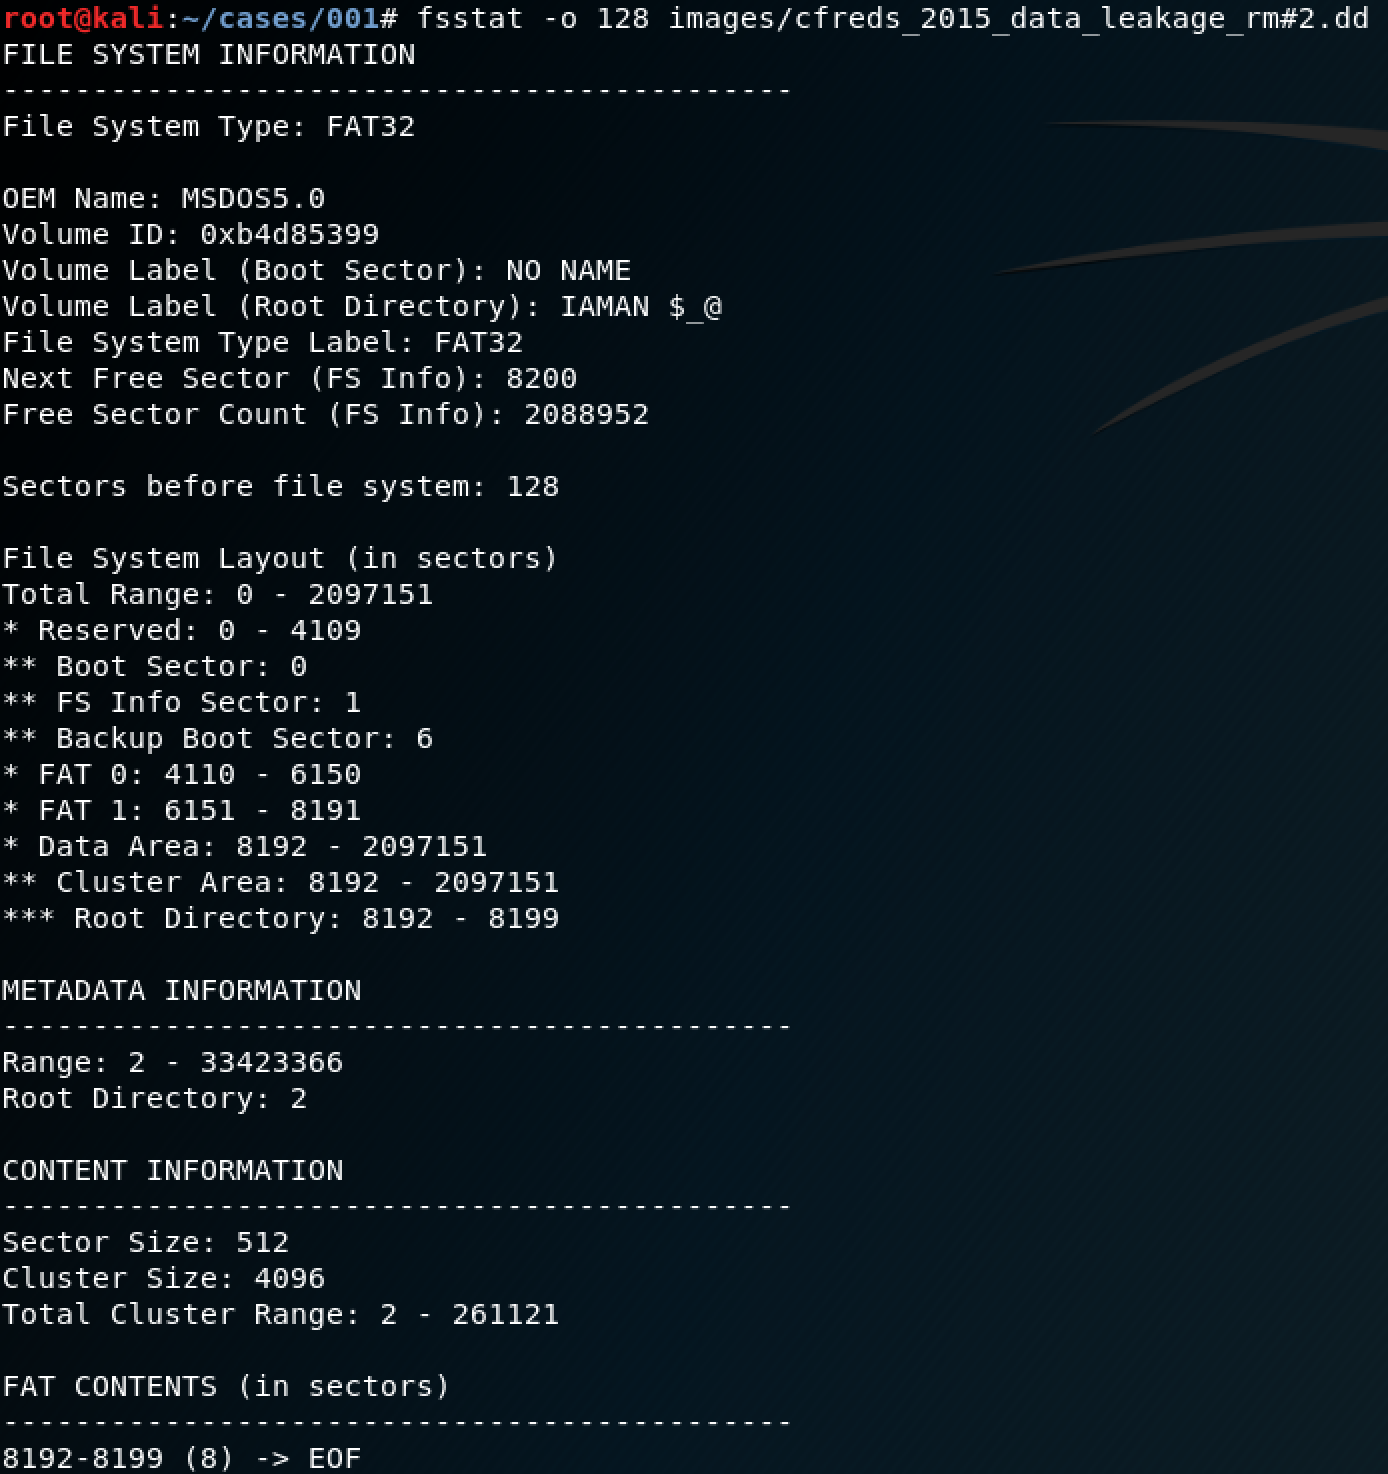
\includegraphics[scale=0.3]{fsstat-output.png}}
					\annotatedFigureBox{-0.0027,0.8905}{0.3133,0.9345}{A}{0.3133,0.8905}%br
					\annotatedFigureBox{-0.0028,0.6505}{0.4153,0.688}{B}{0.4153,0.688}%tr
					\annotatedFigureBox{-0.0032,0.3505}{0.4371,0.632}{C}{0.4371,0.3505}%br
					\annotatedFigureBox{0.0009,0.0865}{0.4343,0.1745}{D}{0.4343,0.0865}%br
					\annotatedFigureBox{0.3938,0.7705}{0.5257,0.8125}{E}{0.5257,0.7705}%br
			\end{annotatedFigure}
		\end{minipage}\hfill
		\begin{minipage}[c]{0.37\textwidth}
			Using TSK's \texttt{fsstat} command with the offset of the file system (-o 128) we are able to view information from three of our FS categories (\textit{file system, metadata, and content}).\\

			\caption{\textbf{File System Info} -- (A) File System Type,\hspace{\textwidth}(B) FS starting Sector,\hspace{\textwidth}(C) FS Layout,\hspace{\textwidth}  (D) Sector {\&} Cluster Address sizes and Cluster Range.\hspace{\textwidth} (E) Root Directory of Volume, name of user.}
			\label{fig:fsstat-output}
		\end{minipage}
	\end{figure}
\end{frame}

\begin{frame}
\frametitle{File Name Information Gathering - \texttt{fls}}
We can extract all the file name pointers, and associated \textit{inode} addresses for files and directories in our disk image.
\begin{figure}[h!t]
\begin{annotatedFigure}
	{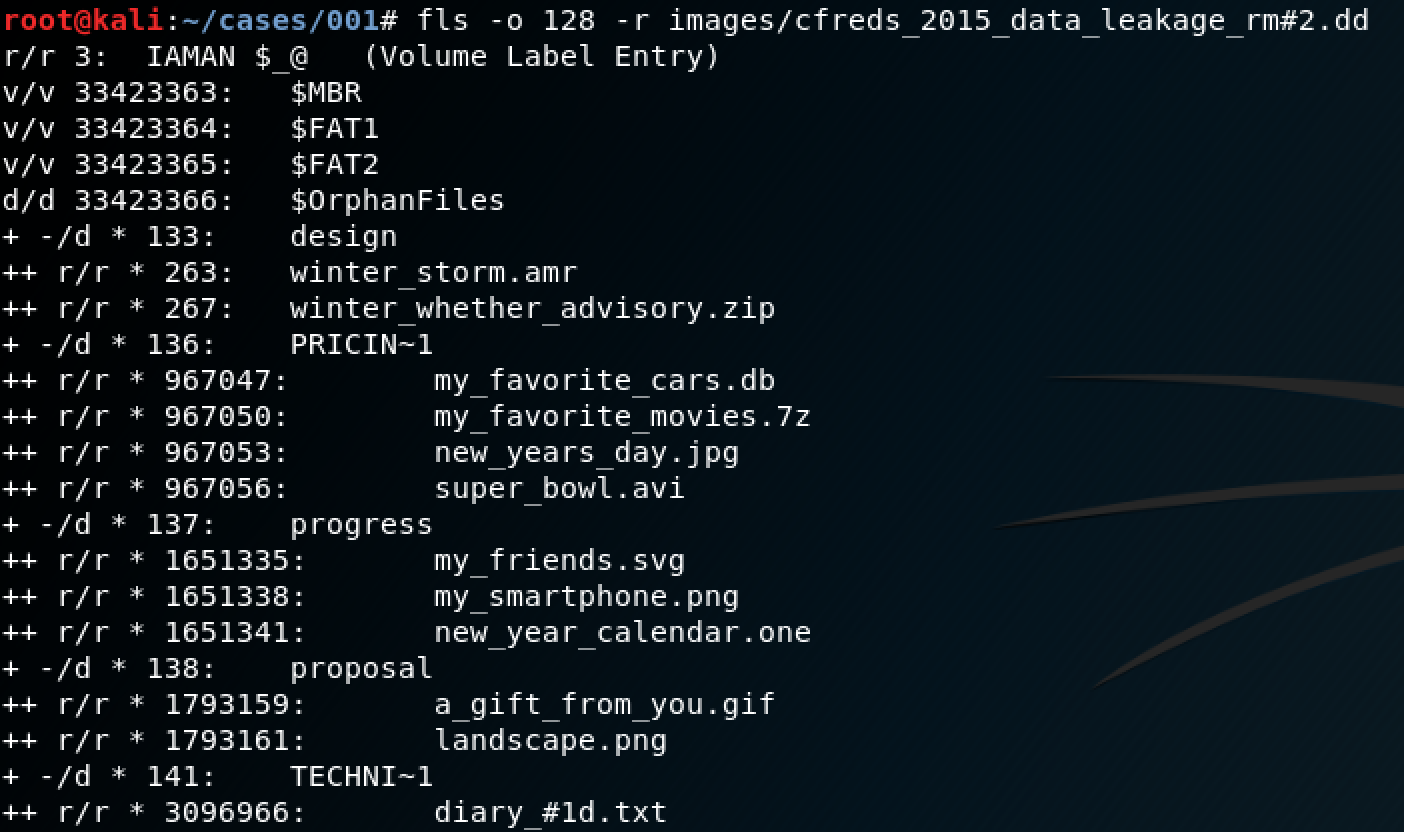
\includegraphics[scale=0.38]{fls-output.png}}
	\annotatedFigureBox{-0.0005,0.7794}{0.2815,0.8739}{A}{0.2815,0.8739}%tr
	\annotatedFigureBox{0.117,0.4655}{0.197,0.5295}{B}{0.117,0.4655}%bl
	\annotatedFigureBox{0.4345,0.9481}{0.4702,1.0014}{C}{0.4345,0.9481}%bl
	\annotatedFigureBox{0.207,0.7355}{0.3655,0.7758}{D}{0.3655,0.7758}%tr
	\annotatedFigureBox{0.0815,0.298}{0.1132,0.3592}{E}{0.1132,0.3592}%tr
\end{annotatedFigure}

\caption{\textbf{File Name Info} -- FAT Tables from physical structure (A), inode address (B), recursively print all file names (C), Unallocated or no longer present files directory - Orphaned Files (D), deleted file indicator (E)}
\label{fig:fls-output}
\end{figure}
\end{frame}

\begin{frame}
\frametitle{Metadata Structure Analysis - \texttt{istat}}
TSK commands starting with an \texttt{i} allow for metadata structure analysis. \texttt{istat} provides metadata details on a particular file given its inode address.
\begin{figure}[h!t]
\begin{annotatedFigure}
	{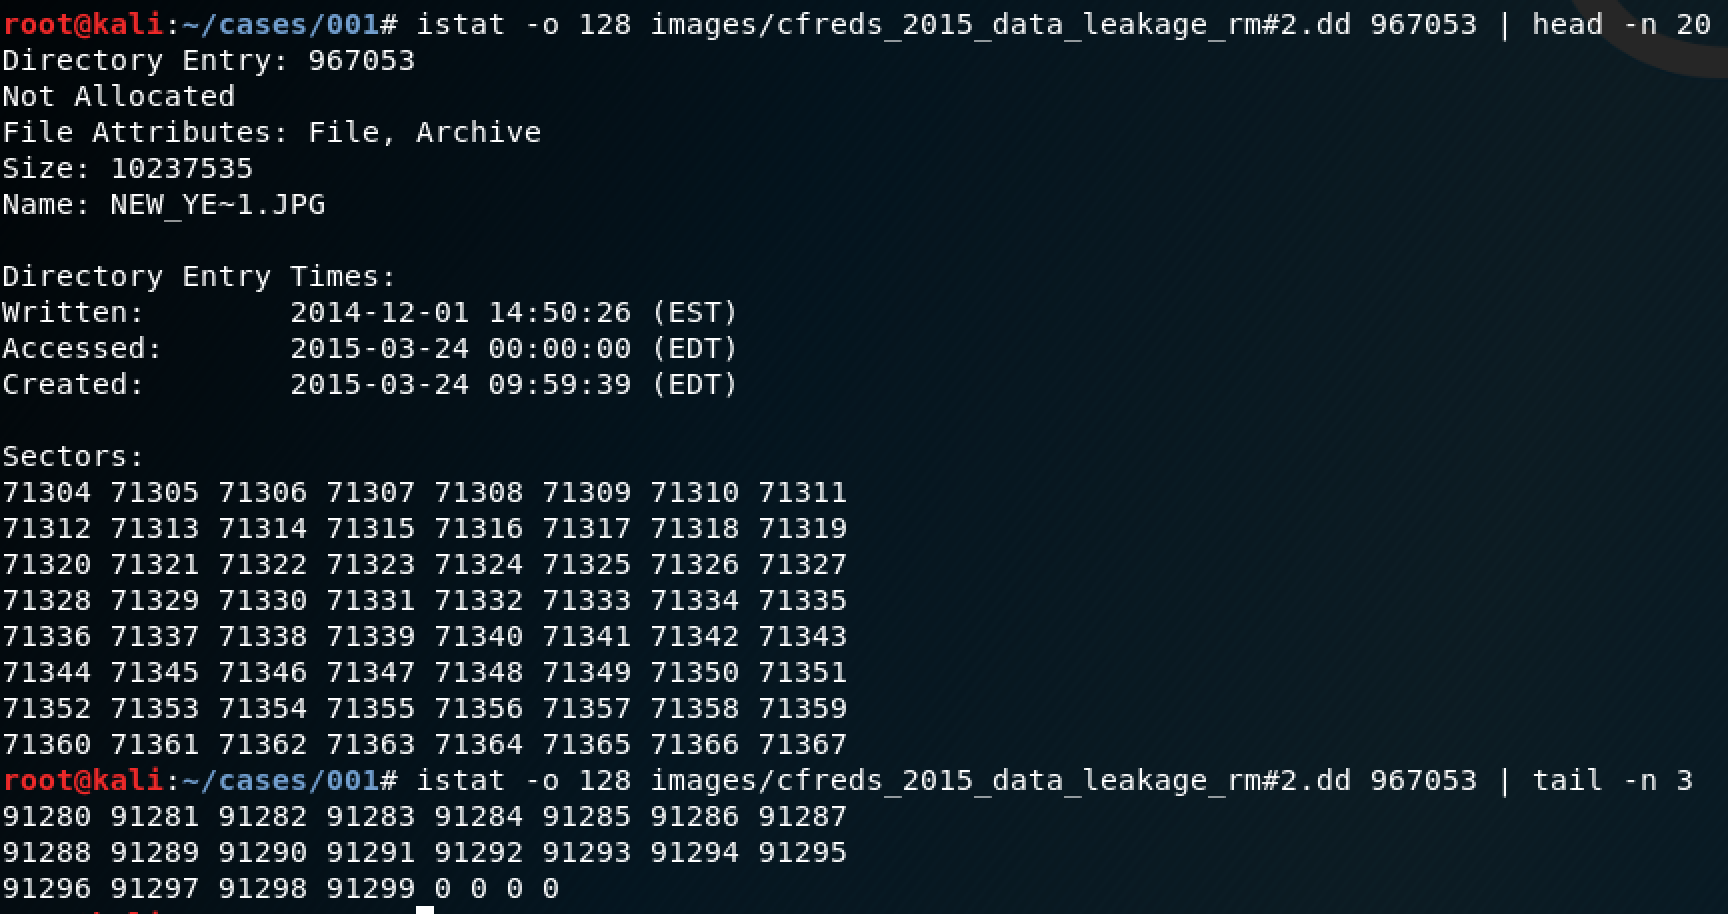
\includegraphics[scale=0.3]{istat-ouput.png}}
	\annotatedFigureBox{0.7875,0.9513}{0.8613,0.9987}{A}{0.8613,0.9513}%br
	\annotatedFigureBox{-0.002,0.872}{0.1485,0.9192}{B}{0.1485,0.872}%br
	\annotatedFigureBox{0.0005,0.7893}{0.1495,0.8426}{C}{0.1495,0.7893}%br
	\annotatedFigureBox{-0.002,0.5467}{0.4358,0.721}{D}{0.4358,0.721}%tr
	\annotatedFigureBox{-0.0015,0.438}{0.0605,0.4863}{E}{0.0605,0.438}%br
	\annotatedFigureBox{0.179,0.0005}{0.2547,0.0459}{F}{0.2547,0.0459}%tr
\end{annotatedFigure}
\caption{\textbf{Metadata Structure info} --  use of inode(A), related file has been deleted (B), file size (C) creation and access times (D), start sector of previously attached data (E), end sector of previously attached data(F).}
\label{fig:istat-output}
\end{figure}
\end{frame}

\begin{frame}
\frametitle{Investigation Sit-rep}
What information have we gathered about this disk image?
\begin{itemize}
\item \textit{File System Architecture:} FAT32
\item \textit{FS starting sector:} 128
\item \textit{Sector ranges for data area clusters:} 8192 to 2097151
\item \textit{Sector Size:} 512
\item \textit{Cluster size:} 4096
\item File names for all deleted files in the FS and their inode numbers
\item Sector Start and End points for any deleted file
\item When the files were created, written and accessed last. (importance of write blockers, and helps with event time-lines).
\end{itemize}
\end{frame}

\begin{frame}[allowframebreaks]
\frametitle{File Recovery From Metadata Structure - \texttt{icat}}
Given the above gathered infomation we can now recover a file, this method uses the data within the metadata structure (inode) to recover the file from disk. 
\begin{figure}[h!t]
\begin{annotatedFigure}
	{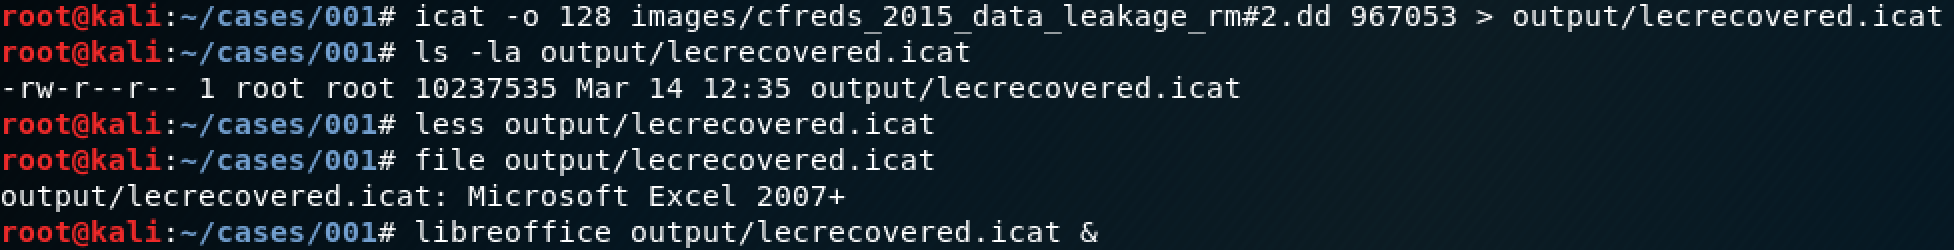
\includegraphics[width=1.0\linewidth]{icat-recovery-output.png}}
	\annotatedFigureBox{-0.0005,0.5799}{0.6505,0.8769}{A}{0.6505,0.5799}%br
	\annotatedFigureBox{-0.006,0.1266}{0.5955,0.4425}{B}{0.5955,0.1266}%br
\end{annotatedFigure}
\caption{\textbf{File Recovery Using Metadata Structure} -- data recovered to file in our OS (A), file type is actually excel, not jpg (B).}
\label{fig:icat-recovery-output}
\end{figure}
\vspace{\baselineskip}

\textit{NOTE:} manual extraction of this file using sector to cluster address conversions and TSK data unit tools (\texttt{blk}*) is possible. This helps when data structures are partial or areas have been overwritten and will be explored in the lab.

	\begin{figure}[h!t]
		{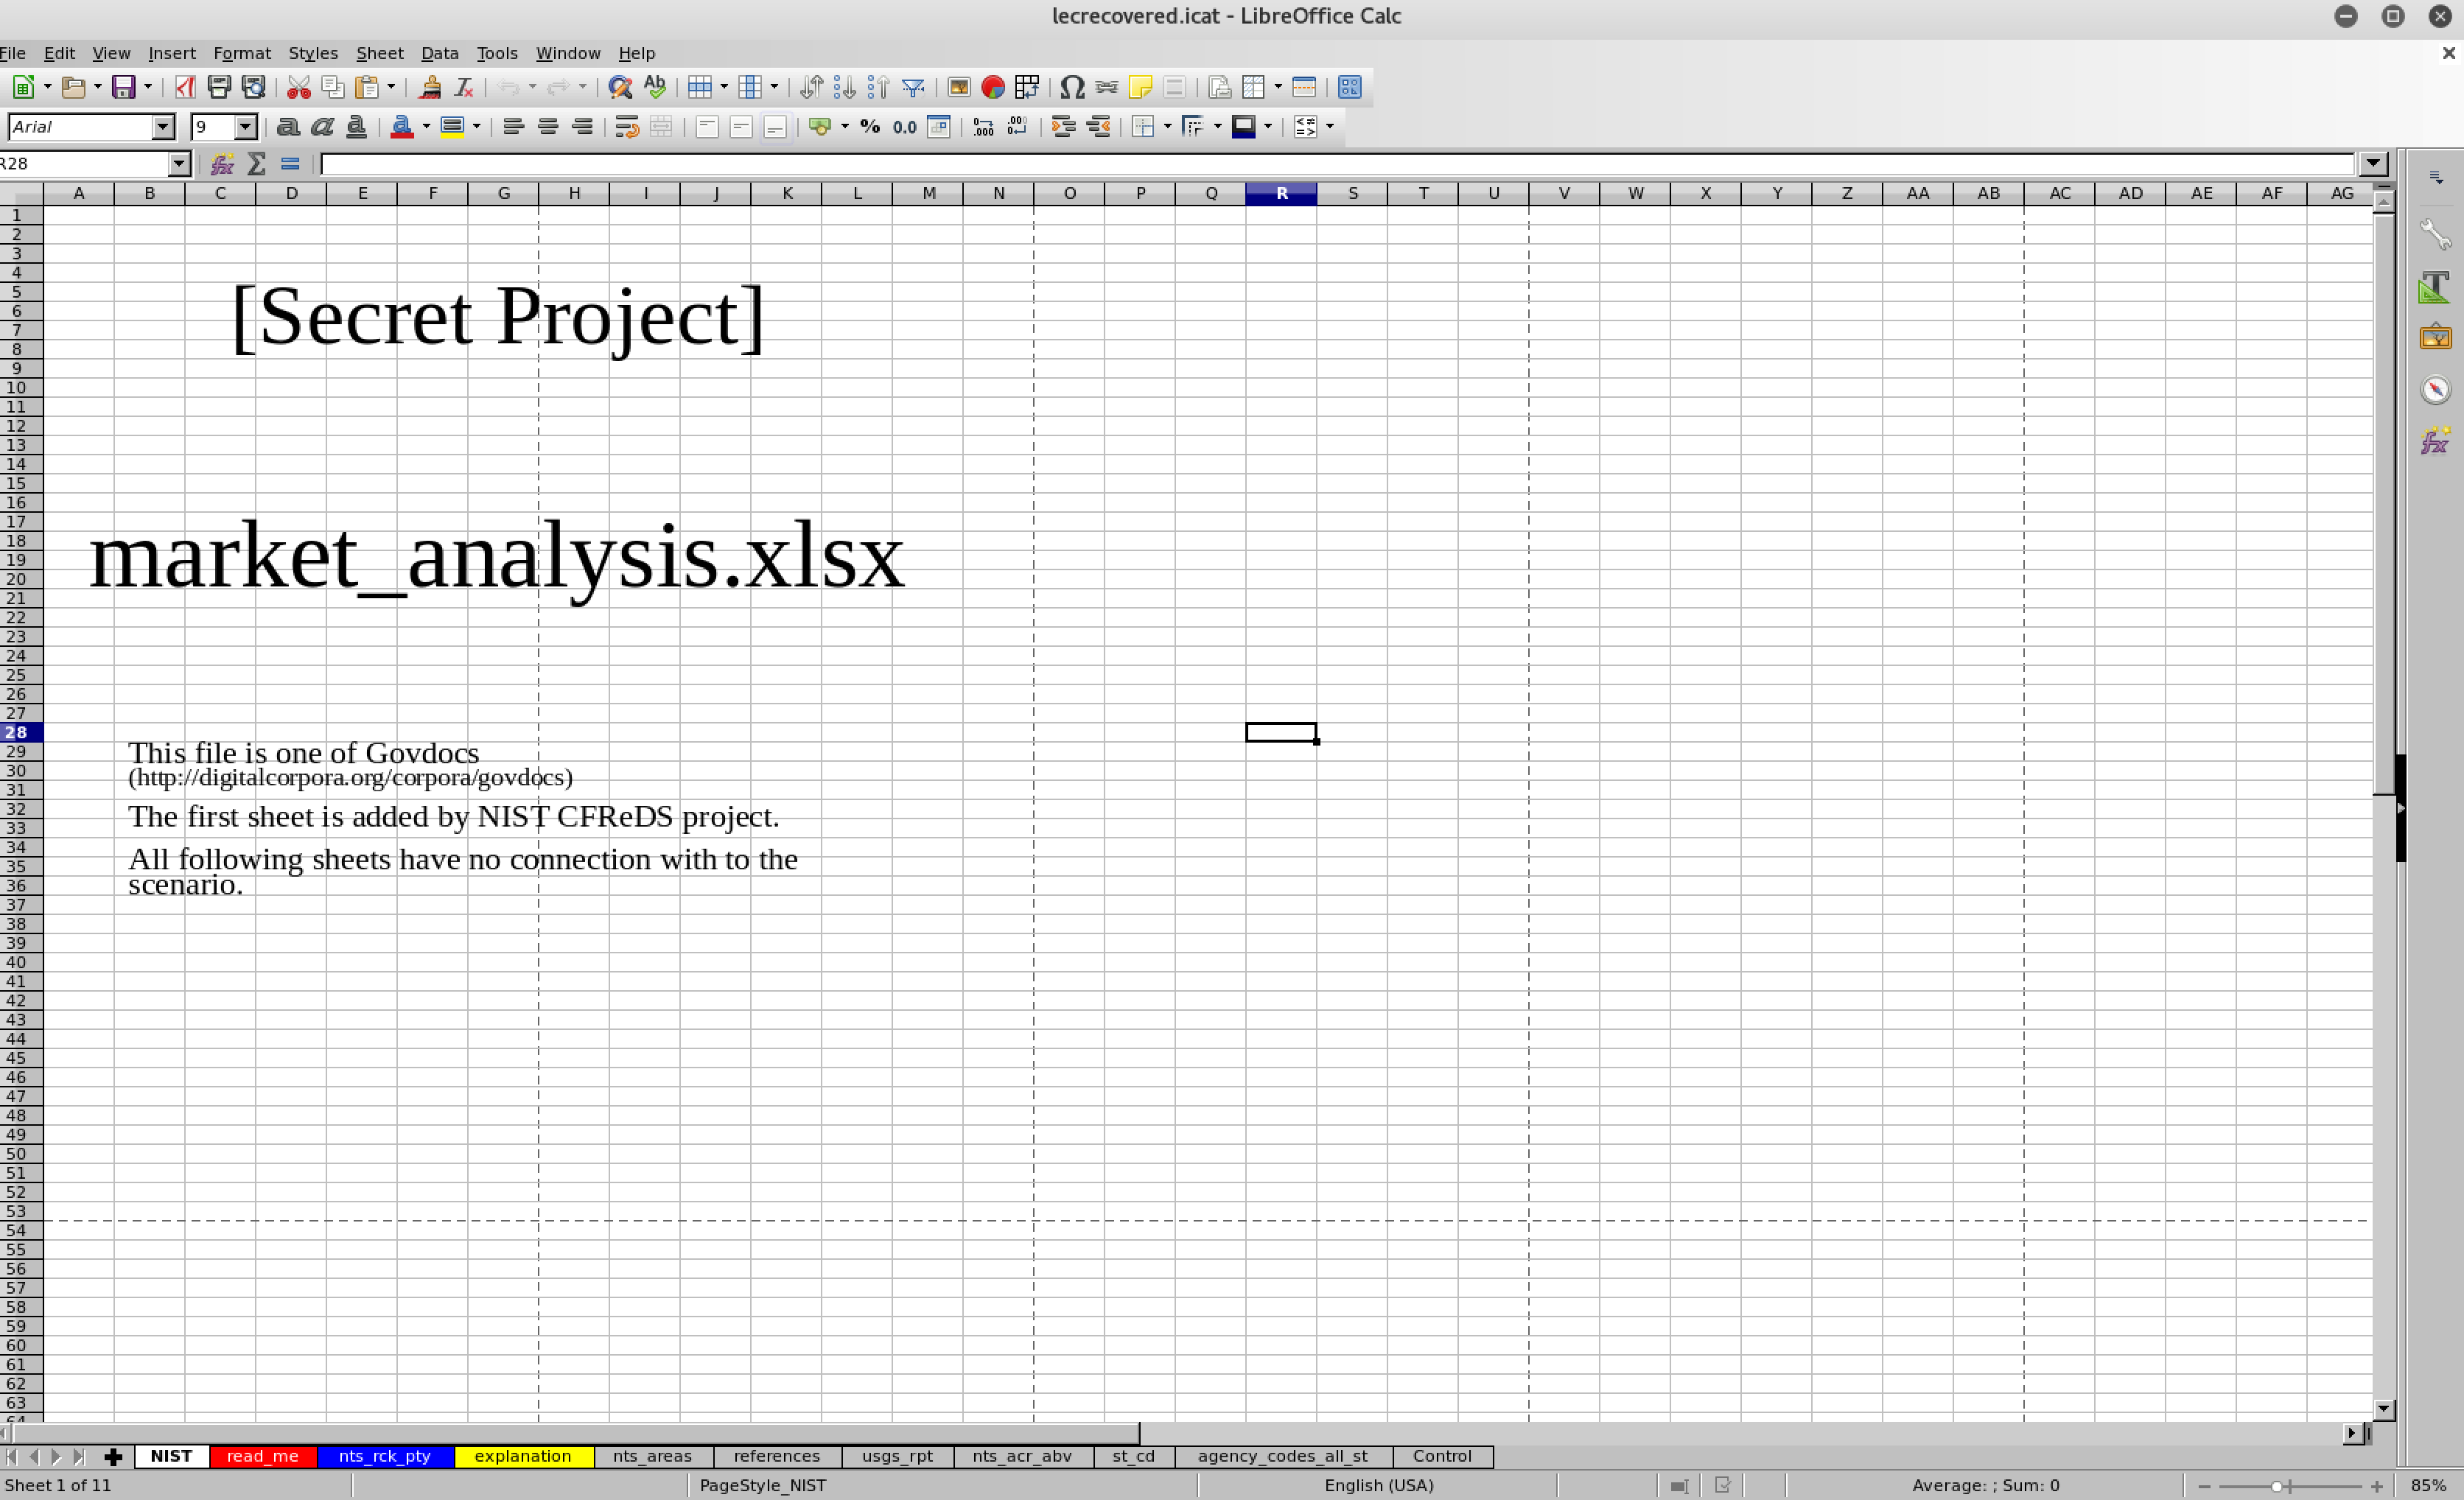
\includegraphics[width=1.0\linewidth]{lecrecovered-open}}
		\caption{Opened Recovered File}
		\label{fig:lecrecovered-open}
	\end{figure}
\end{frame}


\begin{comment}

\begin{frame}
\frametitle{Content Analysis}
\subsection*{Content Analysis}
	\begin{itemize}
		\item \textbf{Data Unit Viewing:} View information in a data unit. We know \textit{where} the evidence could be, but \textbf{not} \textit{what} it is.
		\item \textbf{Logical FS level Searching:} Looks for a specific value or phrase in a \textit{data unit}. We know \textit{what} the content is but \textbf{not} \textit{where}
		\item \textbf{Data Unit Allocation Status:} Verification of each data units status %xtracting and analysing unallocated data in a file system
		\item \textbf{Consistency Check:} Check all allocated data units have 1 metadata entry.\\
		none = orphaned data\\
		2 = unusual {\&} not allowed in file systems.
    \end{itemize}
\end{frame}

\begin{frame}
\frametitle{Metadata Analysis}
\subsection*{Metadata Analysis}
	\begin{itemize}
		\item \textbf{Metadata Lookup:} Reading metadata structure information (istat)
		\item \textbf{Logical File Viewing (data unit):} Looking up the \textit{data units} allocated from metadata and using content lookup to find contents of the file.
			\begin{itemize}
				\item In TSK, the icat tool allows you to view the contents of the data units that are allocated to a metadata structure.\\ 
				-s flag is given, the slack space is shown\\
				-r flag attempts to recover deleted files.
			\end{itemize}
    		\item \textbf{Logical File Searching:} Searches \textit{data units} allocated to a metadata entry
    		\item \textbf{Unallocated Metadata Analysis:} Listing unallocated metadata entries (ils)
    		\item \textbf{Metadata Attribute Aearching {\&} Sorting}
    \end{itemize}
\end{frame}

\begin{frame}
\frametitle{File Name Analysis}
	\subsection*{File Name Analysis}
	\begin{itemize}
		\item \textbf{File Name Listing:} List file and directories looking for data of interest, then investigating further with metadata techniques like logical file viewing.
		\item \textbf{File Name Searching:} If we don't know partial name info like file extension.
    \end{itemize}
\end{frame}

\begin{frame}[allowframebreaks]
	\frametitle{TSK - File System Layer Tools}
	\subsection*{TSK - File System Layer Tools}
	\begin{itemize}
		\item \textbf{fsstat}: shows file system details and statistics including layout, sizes and labels
	\end{itemize}	
	% either swap to live demo or show annotated print screen explaining information shown
	% give exmaple commands
\end{frame}

\begin{frame}
	\frametitle{TSK - File Name Tools}
	\subsection*{TSK -File Name Tools}
	Allow for processing of file name structures.
	\begin{itemize}
		\item \textbf{ffind}: finds allocated and unallocated file names that point to a given meta data structure
		\item \textbf{fls} lists allocated and deleted file names in a directory
	\end{itemize}		
	% either swap to live demo or show annotated print screen explaining information shown
	% give exmaple commands
\end{frame}

\begin{frame}
	\frametitle{TSK - Meta Data Layer Tools}
	\subsection*{TSK - Meta Data Layer Tools}
	\begin{itemize}
		\item \textbf{icat}: Extracts the data units of a file, which is specified by its meta data address.
		\item \textbf{ifind}: Finds the meta data structure that has a given file name pointing to it or the meta data structure that points to a given data unit.
		\item \textbf{ils}: Lists the meta data structures and their contents in a pipe delimited format.
		\item \textbf{istat}: Displays the statistics and details about a given meta data structure in an easy to read format.
	\end{itemize}
	% either swap to live demo or show annotated print screen explaining information shown
	% give exmaple commands
\end{frame}

\begin{frame}
	\frametitle{TSK - Data Unit Tools}
	\subsection*{TSK - Data Unit Tools}
	These file system tools process the data units where file content is stored.
	\begin{itemize}
		\item \textbf{blkcat}: Extracts the contents of a given data unit.
		\item \textbf{blkls}: Lists the details about data units and can extract the unallocated space of the file system.
		\item \textbf{blkstat}: Displays the statistics about a given data unit in an easy to read format.
		\item \textbf{blkcalc}: Calculates where data in the unallocated space image (from blkls) exists in the original image. This is used when evidence is found in unallocated space.
	\end{itemize}
	% either swap to live demo or show annotated print screen explaining information shown
	% give exmaple commands
\end{frame}

\begin{frame}
	\frametitle{TSK - Volume System Tools}
	\subsection*{TSK - Volume System Tools}
	These tools take a disk (or other media) image as input and analyse its partition structures. 
	\begin{itemize}
		\item \textbf{mmls}: Displays the layout of a disk, including the unallocated spaces.
		\item \textbf{mmstat}: Display details about a volume system (typically only the type).
		\item \textbf{mmcat}: Extracts the contents of a specific volume to STDOUT.
	\end{itemize}
	% either swap to live demo or show annotated print screen explaining information shown
	% give exmaple commands
\end{frame}

\end{comment}

\begin{frame}
	\section{Additional Resources}
	\frametitle{Additional Resources}
	\begin{itemize}
	\item \textbf{Books}:
		\begin{itemize}
			\item File System Forensic Analysis- Brian Carrier - \url{http://amzn.eu/1R9U4bz}
			\item Practical Forensic Imaging - Bruce Nikkel - \url{http://amzn.eu/5y057Ba}
		\end{itemize}
	\item \textbf{Reddit}: r/computerforensics \url{https://www.reddit.com/r/computerforensics/wiki/faq}
	\item \textbf{DFRWS Conference}: https://www.dfrws.org/
	\item \textbf{SANS DFIR}:
		\begin{itemize}
			\item \textbf{Blog}: \url{https://digital-forensics.sans.org/blog}
			\item \textbf{Crib Sheets/Posters}: \url{https://digital-forensics.sans.org/community/cheat-sheets}
		\end{itemize}
	\end{itemize}
\end{frame}

\begin{frame}
	\frametitle{Careers}
	\section{Careers}
	\begin{itemize}
		\item \textbf{Police Scotland}\footnote{\tiny\url{http://www.scotland.police.uk/recruitment/police-staff/org-current-vacancies/}}
		\item \textbf{GHCQ} - Internet and Systems Investigation: Forensic Technologist\footnote{\tiny\url{https://recruitmentservices.applicationtrack.com/vx/lang-en-GB/mobile-0/appcentre-3/brand-2/xf-bd8ab30ccf84/candidate/so/pm/1/pl/6/opp/1268}}
		\item \textbf{Cyfor} - eDiscovery Digital Forensics and Cyber Security\footnote{\tiny\url{https://cyfor.co.uk/careers/}}
		\item \textbf{PwC} - Graduate, Technology, eDiscovery {\&} Forensic Computing, Birmingham 2018\footnote{\tiny\url{http://www.careersstudent.pwc.co.uk/ShowJob/Id/882361/Graduate,-Technology,-eDiscovery-Forensic-Computing,-Birmingham-2018/}}
		\item \textbf{Secureworks} - Cyber security and incident response \footnote{\tiny\url{https://www.secureworks.co.uk/careers}}
	\end{itemize}
\end{frame}

\end{document} % End Document